\documentclass[9pt,aspectratio=169]{beamer}
\usetheme[progressbar=none]{metropolis}

\usepackage{amsmath,amssymb}
\usepackage{booktabs}
\usepackage{fontspec}
\setsansfont{Helvetica Neue}

\setbeamertemplate{frame numbering}[fraction]
\setbeamertemplate{navigation symbols}{}
\setbeamertemplate{title separator}{}

\newcommand{\fig}[2][width=\linewidth]{\includegraphics[#1]{../elife/figures/#2}}

\title{Place-field repetition is what a predictive map must do}
\subtitle{when self-motion cannot resolve the symmetry}
\author{Manas Venkata Sai Ravulapalli}
\institute{Ashoka University}
\date{}

\begin{document}

\maketitle

% ------------------------------------------------------------------
\begin{frame}{The puzzle}
\begin{columns}[T]
\begin{column}{0.55\textwidth}
\vspace{10pt}
Place cells in identical compartments fire at the same relative location in every one.

\vspace{14pt}
\begin{quote}
``a high degree of spatial repetition''
\end{quote}
\hfill Spiers et al., 2015

\vspace{18pt}
Usual reading: the hippocampus fails to tell the rooms apart.

\vspace{10pt}
\alert{We show the opposite.}
\end{column}
\begin{column}{0.42\textwidth}
\fig{fig6_brain.pdf}
\end{column}
\end{columns}
\end{frame}

% ------------------------------------------------------------------
\begin{frame}{The claim}
\vspace{10pt}
A network trained only to predict its next observation does not represent physical space $X$.

\vspace{18pt}
\centering
{\Large\alert{It represents the quotient $X/G$.}}

\vspace{22pt}
\raggedright
\begin{itemize}
\item $G$ is the subgroup that self-motion fails to break.
\item Set by equivariance, not by information content.
\end{itemize}
\end{frame}

% ------------------------------------------------------------------
\begin{frame}{Definitions}
\vspace{6pt}
\begin{itemize}
\item \textbf{Orbit}: a set of positions related by the symmetry, e.g.\ $\{x, R^2x\}$ for a
$180^\circ$ rotation.
\vspace{7pt}
\item \textbf{Phase}: which member of the orbit produced the current state.
\vspace{7pt}
\item \textbf{Quotient $X/G$}: physical space $X$ with every orbit collapsed to one point.
\vspace{7pt}
\item \textbf{Invariant}: unchanged under the group, $\phi(h+g) = \phi(h)$.
\vspace{7pt}
\item \textbf{Orbit-phase accuracy}: can a decoder tell which orbit member produced a given
hidden state; chance is $1/|G|$.
\end{itemize}
\end{frame}

% ------------------------------------------------------------------
\begin{frame}{The arenas}
\centering
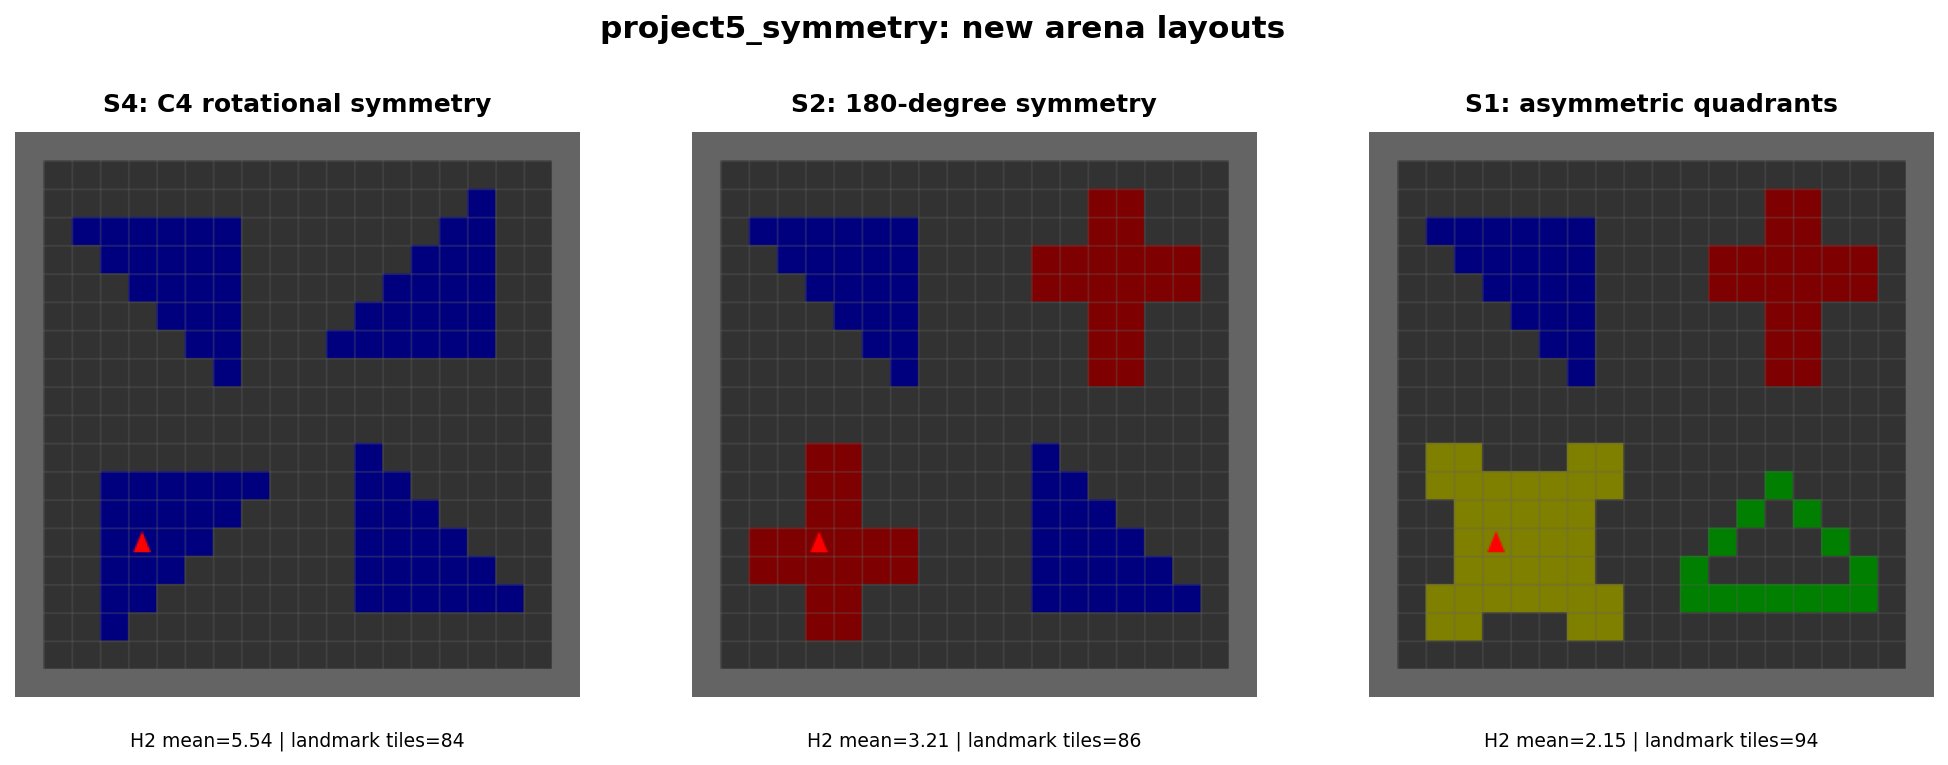
\includegraphics[width=0.85\linewidth]{../images/fig_arenas_overview.png}
\end{frame}

% ------------------------------------------------------------------
\begin{frame}{Architecture and rollout dynamics}
\centering
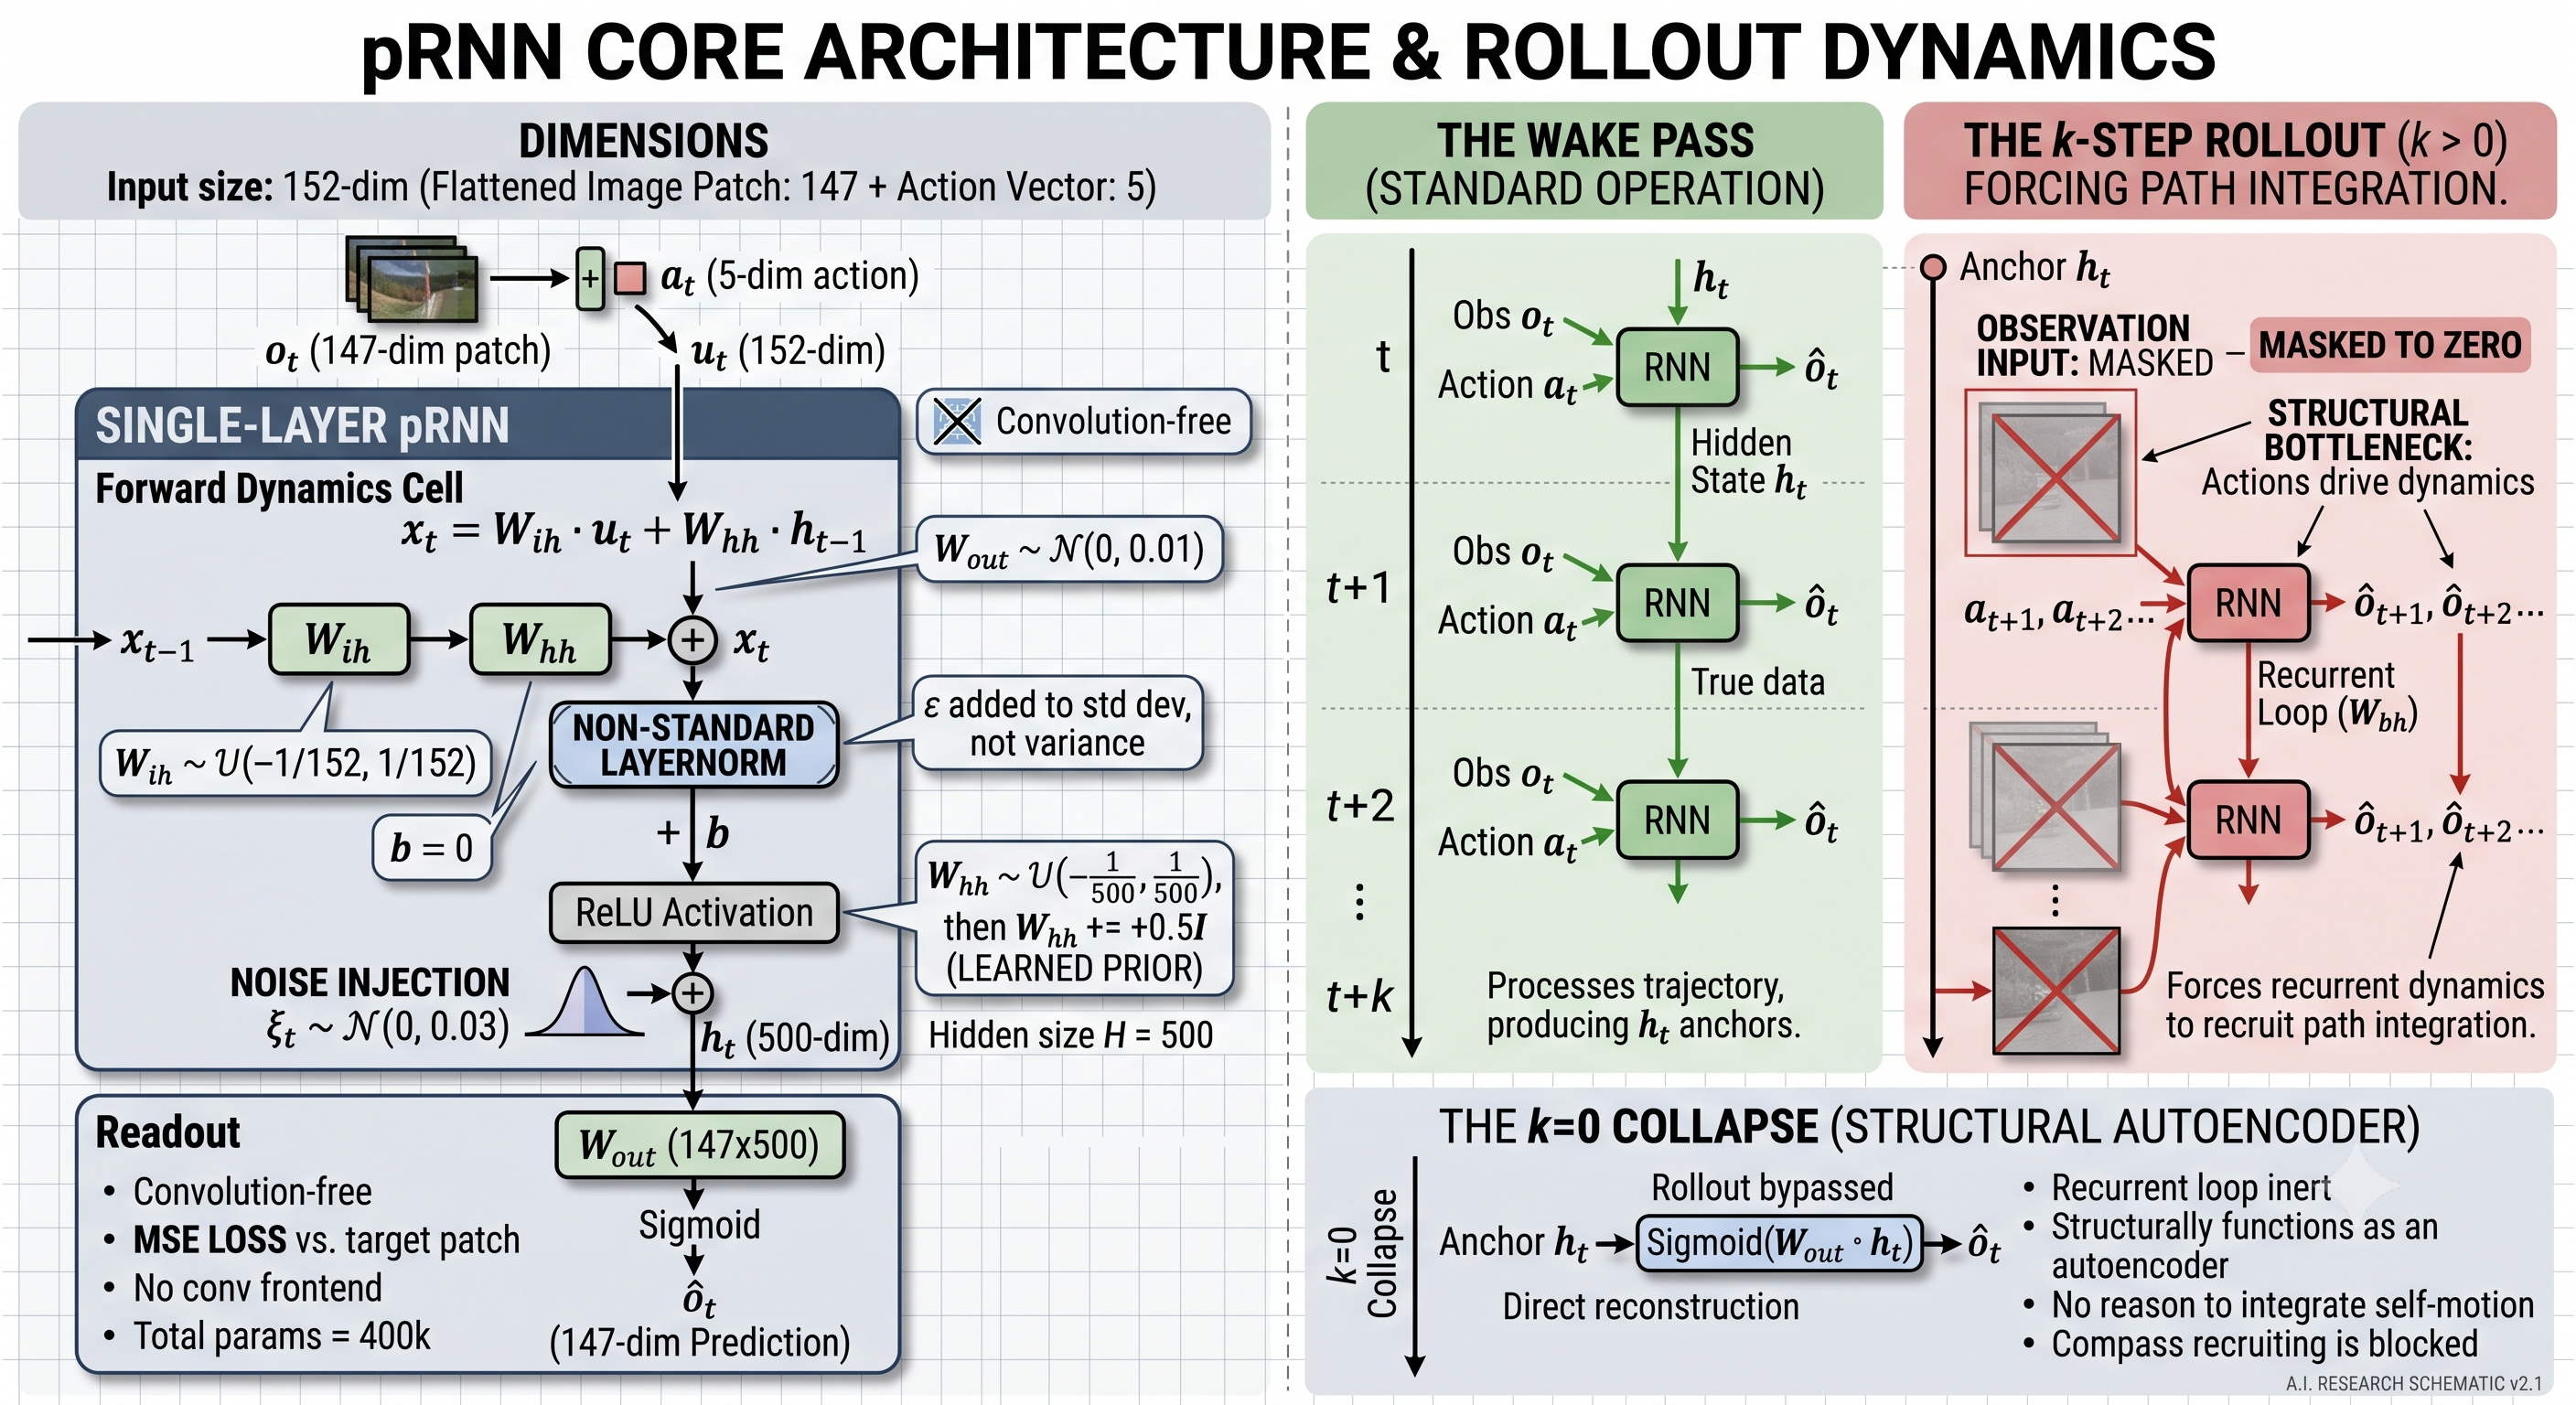
\includegraphics[width=\linewidth]{prnn_schematic.png}
\end{frame}

% ------------------------------------------------------------------
\begin{frame}{The manipulation}
\centering
\fig[height=0.82\textheight]{fig1_setup.pdf}
\end{frame}

% ------------------------------------------------------------------
\begin{frame}{The theorem}
\vspace{6pt}
\begin{block}{Folding onto the quotient}
If the environment has a symmetry $G$ and the head-direction encoding is $G$-invariant, the
posterior over position given any history of observations is $G$-invariant, and no decoder of
the orbit element can beat $1/|G|$.
\end{block}

\vspace{16pt}
An upper bound, not a prediction. Whether a trained network reaches it is empirical.
\end{frame}

% ------------------------------------------------------------------
\begin{frame}{Invariance, not information, folds the code}
\centering
\fig[height=0.66\textheight]{fig2_dissociation.pdf}

\vspace{8pt}
\footnotesize
(a) Each dot is one trained network; can a decoder tell which of two $180^\circ$-related
positions produced this hidden state? \textit{full}/\textit{parity} stay near 1; \textit{axis}/
\textit{const} collapse to chance, only in the symmetric arenas. (b) \textit{axis} and
\textit{parity} carry exactly the same one bit. Indistinguishable in $C_1$; completely
separated in $C_2$. The only difference between them is which one is invariant to the rotation.
\end{frame}

% ------------------------------------------------------------------
\begin{frame}{The $C_4$ ceiling is exactly $1/|G|$}
\centering
\fig[height=0.66\textheight]{fig_ceiling.pdf}

\vspace{8pt}
\footnotesize
Same test, now decoding among 4 rotational copies (chance $1/4$). \textit{axis} is invariant
only under $180^\circ$, so it lands on the $1/2$ ceiling; \textit{const} is invariant under
the full $90^\circ$ rotation, so it lands on $1/4$. The dotted ceilings are computed from
group theory before seeing the data, not fit to it.
\end{frame}

% ------------------------------------------------------------------
\begin{frame}{The fold requires prediction}
\centering
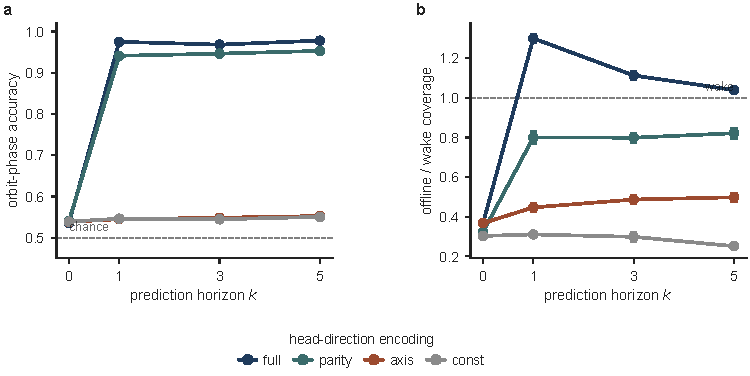
\includegraphics[height=0.6\textheight]{figs/fig_horizon_solo.pdf}

\vspace{8pt}
\footnotesize
$x$-axis is the prediction horizon $k$: how many steps ahead the network is trained to
predict. (a) At $k=0$ (predict the current frame, a pure autoencoder) every encoding sits at
chance. At $k\geq1$ they jump apart and never move again: a step, not a gradient. (b) The same
step in offline replay coverage.
\end{frame}

% ------------------------------------------------------------------
\begin{frame}{Robust, and unaided by any hand-built encoding}
\centering
\fig[width=0.74\linewidth]{fig5_generality.pdf}

\vspace{8pt}
\footnotesize
(a) $x$-axis is what fraction of heading steps are randomly corrupted. \textit{full}/
\textit{parity} degrade smoothly as the compass gets noisier; \textit{axis}/\textit{const}
stay pinned at chance throughout, since corruption doesn't change whether the signal is
invariant. (b) A network given only angular velocity, no absolute heading, still resolves the
asymmetric arena and still folds the symmetric one, with no invariant encoding built in by
hand.
\end{frame}

% ------------------------------------------------------------------
\begin{frame}{The same law explains the animal data}
\vspace{4pt}
\begin{columns}[T]
\begin{column}{0.48\textwidth}
\textbf{Neural}

\vspace{4pt}
\centering
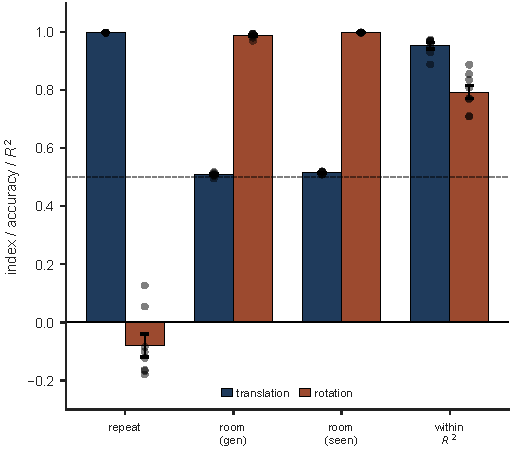
\includegraphics[width=0.92\linewidth]{figs/fig_compartments_solo.pdf}

\vspace{2pt}
\raggedright
\footnotesize
Translated compartments: fields repeat, room undecodable. Rotated compartments: repetition
vanishes, room decodes perfectly. Grieves et al., 2016.
\end{column}
\begin{column}{0.48\textwidth}
\textbf{Behavioral}

\vspace{6pt}
\small
A separate cohort learned to tell the rooms apart.

\vspace{6pt}
Learning was significantly impaired exactly where the neural code folds.

\vspace{6pt}
\alert{``place field repetition constrains spatial learning''}
\end{column}
\end{columns}
\end{frame}

% ------------------------------------------------------------------
\begin{frame}{The fold, seen geometrically}
\centering
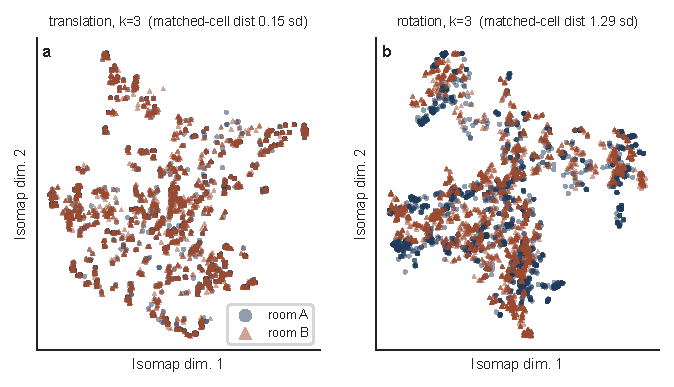
\includegraphics[height=0.66\textheight]{../biorxiv/figures/fig_isomap_manifold.pdf}

\vspace{4pt}
\footnotesize
Isomap embedding, no decoder involved (Levenstein et al.\ style). Colour is room identity, never
shown to Isomap. Matched-cell distance in the embedding: $0.13$ vs.\ $1.31$ (embedding-spread
units), $n=8$ each, $p=1.6\times10^{-4}$.
\end{frame}

% ------------------------------------------------------------------
\begin{frame}{Theoretical grounding}
\vspace{10pt}
\begin{itemize}
\item The belief process descends to a Markov process on $X/G$: a MDP homomorphism.
\vspace{8pt}
\item States that share the same future are bisimilar; this is a bisimulation relation.
\vspace{8pt}
\item A predictive learner acquiring the successor representation of its belief state should
represent that quotient, with no reward and no group given to the network.
\end{itemize}
\end{frame}

% ------------------------------------------------------------------
\begin{frame}{Summary}
\vspace{12pt}
\begin{itemize}
\item A predictive map represents a quotient $X/G$, not physical space $X$.
\vspace{6pt}
\item Proved as a ceiling, saturated only under a predictive objective.
\vspace{6pt}
\item One principle explains repetition, neurally and behaviorally.
\vspace{6pt}
\item One architecture, one real-neuron test that is consistent with the quotient, not proof
of it.
\end{itemize}

\vspace{20pt}
\centering
\large A cognitive map represents space only up to the symmetries its own motion cannot break.
\end{frame}

% ==================================================================
% APPENDIX --- for Hasselmo. Not part of the talk; pull up if asked.
% ==================================================================
\appendix

\begin{frame}{You already built the compass this theory needs}
\vspace{6pt}
LaChance \& Hasselmo, \textit{Nat Commun} \textbf{15}:8025 (2024). Two identical cue cards, on
opposite walls of a square --- a symmetry the visual scene cannot break.

\vspace{10pt}
\centering
\begin{tabular}{lcc}
\toprule
head-direction cells & become bidirectional? & \\
\midrule
postrhinal (POR)     & \textbf{yes} & $p = 2\times10^{-10}$ \\
retrosplenial (RSC)  & \textbf{yes} & $p = 1.4\times10^{-4}$ \\
entorhinal (MEC/PaS) & no           & $p = 0.62$ \\
\bottomrule
\end{tabular}

\vspace{14pt}
\raggedright
A bidirectional head-direction cell \emph{is} a $C_2$-invariant compass: it reports the same heading
at $x$ and at $R_{180}x$.

\vspace{6pt}
Zhang, Grieves \& Jeffery (2022) get the same object by varying the environment: RSC tuning is
unidirectional in a circle, \textbf{bi}directional in a $C_2$ box, \textbf{tetra}directional in a
$C_4$ box.

\vspace{10pt}
\centering
\alert{Neither paper recorded a single place cell.}
\end{frame}

% ------------------------------------------------------------------
\begin{frame}{We have that compass, and it is the \emph{only} thing that matters}
\vspace{4pt}
Orbit-phase decoding: can a decoder say \emph{which} of two $180^\circ$-related positions the animal
occupies? Chance $=0.500$. One dot per network, $n \approx 10$.

\vspace{8pt}
\centering
\begin{tabular}{lcccc}
\toprule
arena & \textit{full} & \textit{parity} & \textit{axis} & \textit{const} \\
\midrule
$C_1$ (no symmetry) & 0.981 & 0.972 & 0.971 & 0.966 \\
$C_2$               & 0.978 & 0.955 & \textbf{0.552} & \textbf{0.552} \\
$C_4$               & 0.984 & 0.933 & \textbf{0.544} & \textbf{0.521} \\
\bottomrule
\end{tabular}

\vspace{12pt}
\raggedright
\textit{axis} $=\{E,W\}$ vs $\{N,S\}$ --- \textbf{invariant} under $180^\circ$.\\
\textit{parity} $=\{E,S\}$ vs $\{W,N\}$ --- \textbf{breaks} $180^\circ$.

\vspace{6pt}
\alert{Both carry exactly one bit of heading.} Same information, same architecture, same walls, same
corners, same boundary cells. Opposite folds.

\vspace{6pt}
No boundary-vector model can state this: it has no representation of \emph{which} bit the compass
carries. Nor can any animal experiment run it.
\end{frame}

% ------------------------------------------------------------------
\begin{frame}{It is the objective, not the assumptions}
\vspace{4pt}
Same network, same compass, same inputs. Only the rollout horizon $k$ changes. At $k=0$ the target is
the network's own current observation --- a pure autoencoder.

\vspace{8pt}
\centering
\begin{tabular}{lccccc}
\toprule
$k$ & \textit{full} & \textit{parity} & \textit{axis} & \textit{const} & \textit{axis} vs \textit{parity} \\
\midrule
0 (autoencoder) & 0.536 & 0.541 & 0.539 & 0.539 & $p = 0.59$ \\
1               & \textbf{0.975} & \textbf{0.941} & 0.545 & 0.546 & $p = 0.002$ \\
5               & 0.978 & 0.953 & 0.553 & 0.551 & $p = 0.002$ \\
\bottomrule
\end{tabular}

\vspace{12pt}
\raggedright
At $k=0$ the compass is \emph{right there} --- the input alone separates 1228 of 1296 states --- and
the network \alert{discards it}. All four encodings sit at chance. \textit{axis} and \textit{parity}
are indistinguishable.

\vspace{6pt}
\textbf{One step of prediction} makes heading load-bearing.

\vspace{6pt}
Reconstructing what you see never requires knowing which of two identical rooms you are in.
Predicting what you will see next does.
\end{frame}

% ------------------------------------------------------------------
\begin{frame}{The experiment, and it is yours to run}
\vspace{10pt}
\centering
\Large
Record place cells in the square, with \textbf{two identical opposing cue cards}.

\vspace{16pt}
\normalsize
\raggedright
\textbf{Prediction, no free parameters:}
\begin{itemize}
\item $C_2$ place-field repetition --- fields recur at $180^\circ$-related locations.
\item A decoder for \emph{which half} of the arena the animal occupies is bounded at
$\tfrac{1}{2}$.
\end{itemize}

\vspace{10pt}
\textbf{Why it is a real test:} your MEC head-direction cells did \emph{not} go bidirectional
($p=0.62$) and your grid cells did not change. If the hippocampus reads only that channel, nothing
happens --- and we are wrong. But POR's densest hippocampal projection is to \emph{subiculum}, and
the LMN lesion (Harland 2017) \emph{does} fold hippocampal fields.

\vspace{10pt}
\alert{The apparatus already exists. A null falsifies us.}
\end{frame}

\end{document}
